%%%%%%%%%%%%%%%%%%%%%%%%%%%%%%%%%%%%%%%%%
% Lachaise Assignment
% LaTeX Template
% Version 1.0 (26/6/2018)
%
% This template originates from:
% http://www.LaTeXTemplates.com
%
% Authors:
% Marion Lachaise & François Févotte
% Vel (vel@LaTeXTemplates.com)
%
% License:
% CC BY-NC-SA 3.0 (http://creativecommons.org/licenses/by-nc-sa/3.0/)
% 
%%%%%%%%%%%%%%%%%%%%%%%%%%%%%%%%%%%%%%%%%

%----------------------------------------------------------------------------------------
%	PACKAGES AND OTHER DOCUMENT CONFIGURATIONS
%----------------------------------------------------------------------------------------

\documentclass{article}

%%%%%%%%%%%%%%%%%%%%%%%%%%%%%%%%%%%%%%%%%
% Lachaise Assignment
% Structure Specification File
% Version 1.0 (26/6/2018)
%
% This template originates from:
% http://www.LaTeXTemplates.com
%
% Authors:
% Marion Lachaise & François Févotte
% Vel (vel@LaTeXTemplates.com)
%
% License:
% CC BY-NC-SA 3.0 (http://creativecommons.org/licenses/by-nc-sa/3.0/)
% 
%%%%%%%%%%%%%%%%%%%%%%%%%%%%%%%%%%%%%%%%%

%----------------------------------------------------------------------------------------
%	PACKAGES AND OTHER DOCUMENT CONFIGURATIONS
%----------------------------------------------------------------------------------------
\usepackage{listings}
\usepackage{amsmath,amsfonts,stmaryrd,amssymb} % Math packages
\usepackage{amsthm}

\usepackage{enumerate} % Custom item numbers for enumerations

\usepackage[linesnumbered,ruled,vlined]{algorithm2e} % Algorithms

\usepackage[framemethod=tikz]{mdframed} % Allows defining custom boxed/framed environments
\usepackage{subfigure}
\usepackage{listings} % File listings, with syntax highlighting
\usepackage{booktabs}
\usepackage{diagbox}

\lstset{
	basicstyle=\ttfamily, % Typeset listings in monospace font
}

%----------------------------------------------------------------------------------------
%	DOCUMENT MARGINS
%----------------------------------------------------------------------------------------

\usepackage{geometry} % Required for adjusting page dimensions and margins

\geometry{
	paper=a4paper, % Paper size, change to letterpaper for US letter size
	top=2.5cm, % Top margin
	bottom=3cm, % Bottom margin
	left=2.5cm, % Left margin
	right=2.5cm, % Right margin
	headheight=14pt, % Header height
	footskip=1.5cm, % Space from the bottom margin to the baseline of the footer
	headsep=1.2cm, % Space from the top margin to the baseline of the header
	%showframe, % Uncomment to show how the type block is set on the page
}

%----------------------------------------------------------------------------------------
%	FONTS
%----------------------------------------------------------------------------------------

\usepackage[utf8]{inputenc} % Required for inputting international characters
\usepackage[T1]{fontenc} % Output font encoding for international characters
% \usepackage{XCharter} % Use the XCharter fonts
\usepackage{CTEX}
\usepackage[hidelinks]{hyperref}

%----------------------------------------------------------------------------------------
%	COMMAND LINE ENVIRONMENT
%----------------------------------------------------------------------------------------

% Usage:
% \begin{commandline}
%	\begin{verbatim}
%		$ ls
%		
%		Applications	Desktop	...
%	\end{verbatim}
% \end{commandline}

\mdfdefinestyle{commandline}{
	leftmargin=10pt,
	rightmargin=10pt,
	innerleftmargin=15pt,
	middlelinecolor=black!50!white,
	middlelinewidth=2pt,
	frametitlerule=false,
	backgroundcolor=black!5!white,
	frametitle={Command Line},
	frametitlefont={\normalfont\sffamily\color{white}\hspace{-1em}},
	frametitlebackgroundcolor=black!50!white,
	nobreak,
}

% Define a custom environment for command-line snapshots
\newenvironment{commandline}{
	\medskip
	\begin{mdframed}[style=commandline]
}{
	\end{mdframed}
	\medskip
}

%----------------------------------------------------------------------------------------
%	FILE CONTENTS ENVIRONMENT
%----------------------------------------------------------------------------------------

% Usage:
% \begin{file}[optional filename, defaults to "File"]
%	File contents, for example, with a listings environment
% \end{file}

\mdfdefinestyle{file}{
	innertopmargin=1.6\baselineskip,
	innerbottommargin=0.8\baselineskip,
	topline=false, bottomline=false,
	leftline=false, rightline=false,
	leftmargin=2cm,
	rightmargin=2cm,
	singleextra={%
		\draw[fill=black!10!white](P)++(0,-1.2em)rectangle(P-|O);
		\node[anchor=north west]
		at(P-|O){\ttfamily\mdfilename};
		%
		\def\l{3em}
		\draw(O-|P)++(-\l,0)--++(\l,\l)--(P)--(P-|O)--(O)--cycle;
		\draw(O-|P)++(-\l,0)--++(0,\l)--++(\l,0);
	},
	nobreak,
}

% Define a custom environment for file contents
\newenvironment{file}[1][File]{ % Set the default filename to "File"
	\medskip
	\newcommand{\mdfilename}{#1}
	\begin{mdframed}[style=file]
}{
	\end{mdframed}
	\medskip
}

%----------------------------------------------------------------------------------------
%	NUMBERED QUESTIONS ENVIRONMENT
%----------------------------------------------------------------------------------------

% Usage:
% \begin{question}[optional title]
%	Question contents
% \end{question}

\mdfdefinestyle{question}{
	innertopmargin=1.2\baselineskip,
	innerbottommargin=0.8\baselineskip,
	roundcorner=5pt,
	nobreak,
	singleextra={%
		\draw(P-|O)node[xshift=1em,anchor=west,fill=white,draw,rounded corners=5pt]{%
		Question \theQuestion\questionTitle};
	},
}

\newcounter{Question} % Stores the current question number that gets iterated with each new question

% Define a custom environment for numbered questions
\newenvironment{question}[1][\unskip]{
	\bigskip
	\stepcounter{Question}
	\newcommand{\questionTitle}{~#1}
	\begin{mdframed}[style=question]
}{
	\end{mdframed}
	\medskip
}

%----------------------------------------------------------------------------------------
%	WARNING TEXT ENVIRONMENT
%----------------------------------------------------------------------------------------

% Usage:
% \begin{warn}[optional title, defaults to "Warning:"]
%	Contents
% \end{warn}

\mdfdefinestyle{warning}{
	topline=false, bottomline=false,
	leftline=false, rightline=false,
	nobreak,
	singleextra={%
		\draw(P-|O)++(-0.5em,0)node(tmp1){};
		\draw(P-|O)++(0.5em,0)node(tmp2){};
		\fill[black,rotate around={45:(P-|O)}](tmp1)rectangle(tmp2);
		\node at(P-|O){\color{white}\scriptsize\bf !};
		\draw[very thick](P-|O)++(0,-1em)--(O);%--(O-|P);
	}
}

% Define a custom environment for warning text
\newenvironment{warn}[1][Warning:]{ % Set the default warning to "Warning:"
	\medskip
	\begin{mdframed}[style=warning]
		\noindent{\textbf{#1}}
}{
	\end{mdframed}
}

%----------------------------------------------------------------------------------------
%	INFORMATION ENVIRONMENT
%----------------------------------------------------------------------------------------

% Usage:
% \begin{info}[optional title, defaults to "Info:"]
% 	contents
% 	\end{info}

\mdfdefinestyle{info}{%
	topline=false, bottomline=false,
	leftline=false, rightline=false,
	nobreak,
	singleextra={%
		\fill[black](P-|O)circle[radius=0.4em];
		\node at(P-|O){\color{white}\scriptsize\bf i};
		\draw[very thick](P-|O)++(0,-0.8em)--(O);%--(O-|P);
	}
}

% Define a custom environment for information
\newenvironment{info}[1][Info:]{ % Set the default title to "Info:"
	\medskip
	\begin{mdframed}[style=info]
		\noindent{\textbf{#1}}
}{
	\end{mdframed}
}
 % Include the file specifying the document structure and custom commands

%----------------------------------------------------------------------------------------
%	ASSIGNMENT INFORMATION
%----------------------------------------------------------------------------------------

\title{Reinforcement Learning Final Project} % Title of the assignment

\author{pangbo} % Author name and email address

\date{\today} % University, school and/or department name(s) and a date

%----------------------------------------------------------------------------------------

\begin{document}

\maketitle % Print the title

%----------------------------------------------------------------------------------------
%	INTRODUCTION
%----------------------------------------------------------------------------------------

\section{Value-based Reinforcement Learning}

\subsection{方法}

基于价值的强化学习是一种强化学习方法,其核心思想是通过对价值函数进行建模和估计,以此为依据制定策略。在训练阶段,其学习目标是学到一个函数,知道当前状态和动作之后,这个函数可以输出状态下这个动作所能带来的长期价值期望,记为Q值。

在决策阶段,我们可以根据训练好的函数,在一个新的状态下,尝试可选动作集合中的每一个动作,最终采取Q值最大的动作,这样就可以带来最大的长期收益。

DQN是基于价值的强化学习的一个典型代表,其核心思想是通过神经网络来估计Q值函数。在训练阶段,我们通过神经网络来估计Q值函数,然后通过Q值函数来制定策略。在决策阶段,我们可以根据训练好的神经网络,在一个给定状态下,采取Q值最大的动作。

原始DQN在实际运用中面临的一大挑战是难以收敛,因此,研究人员提出了许多改进方法以提高DQN的性能。

\subsubsection{Double Q-learning}

原始DQN的更新公式如下:
\begin{equation}
	Q(s_t, a_t) \leftarrow r_{t+1} + \max_{a} Q(s_{t+1}, a)
	\label{eq:q-learning}
\end{equation}

可以看出,原始DQN需要使用Q函数的值来更新Q函数,而Q函数是在更新过程中不断变化的,这导致神经网络的训练目标不断变化,不利于神经网络的收敛。另一个问题在于,Q函数可能高估某些动作的Q值,而使用单个Q函数进行训练的方式难以修复这种问题。

为解决这些问题,研究人员提出了Double Q-learning的方法。Double Q-learning的核心思想是使用两个Q函数来分别估计Q值,然后使用其中一个Q函数来选择动作,使用另一个Q函数来估计Q值。两个Q函数轮流进行更新。具体来说,Double Q-learning的更新公式如下:

\begin{equation}
	Q(s_t, a_t) \leftarrow r_{t+1} + Q'\left(s_t,\arg\max_{a} Q(s_{t+1}, a)\right)
	\label{eq:double-q-learning}
\end{equation}

\subsubsection{Dueling DQN}

Dueling DQN的核心思想是将Q函数分解为状态值函数和优势函数,即:

\begin{equation}
	Q(s, a) = V(s) + A(s, a)
	\label{eq:dueling-dqn}
\end{equation}

其中,$V(s)$表示状态值函数,$A(s, a)$表示优势函数。状态值函数表示状态$s$自身的价值,而优势函数表示在状态$s$下,采取动作$a$相对于采取其他动作所能带来的长期收益的期望。

Dueling DQN可以更好地对状态价值进行评估,拥有更快的学习速度和更好的收敛性。在具有多个冗余或者近似的动作时,Dueling DQN可以比DQN更快的识别出策正确动作。

\subsubsection{Multi-step Learning}

Q-learning一般使用时序差分(Temporal Difference)的方法来更新Q值,即只考虑下一步的Q值。Multi-step Learning的核心思想是在更新Q值时,不仅考虑下一步的Q值,而是考虑未来多步的Q值。Multi-step Learning是一种介于时序差分与蒙特卡洛方法之间的方法,可以更好地平衡学习速度和收敛性。其更新公式如下:

\begin{equation}
	Q(s_t, a_t) \leftarrow \sum^{m}_{i=1}\gamma^{i-1} r_{t+i} + \max_{a} Q(s_{t+m}, a)
	\label{eq:multi-step-learning}
\end{equation}

\subsubsection{Noisy Net}

在DQN的训练过程中,我们需要不断地探索新的状态和动作,以便更好地估计Q值函数。$\epsilon$-greedy方法是一种常用的探索方法,其核心思想是以$\epsilon$的概率随机选择动作,以$1-\epsilon$的概率选择Q值最大的动作。在刚开始训练时,我们需要大量地探索新的状态和动作,因此$\epsilon$的值需要设置的较大,随着训练的进行,我们需要逐渐减小$\epsilon$的值,以便更多地选择Q值最大的动作。

Noisy Net的核心思想是直接在神经网络中引入噪声,以便更好地探索新的状态和动作。相较于$\epsilon$-greedy方法,Noisy Net拥有更大的不确定性、更好的探索性和更快的收敛性。

\subsubsection{Prioritized Experience Replay}

在DQN的训练过程中,我们需要不断地从历史回放中均匀随机采样,以便训练神经网络。Prioritized Experience Replay的核心思想是在采样时,不再是均匀随机采样,而是根据经验的优先级进行采样。样本的优先级可以根据样本在训练过程中的损失计算,即每一轮从Replay Buffer中选择样本输入模型后,使用模型预测结果的损失反过来更新该样本的优先级,损失越大,优先级越高。总而言之,Prioritized Experience Replay可以更好地利用经验,提高训练效率。

\subsubsection{Rainbow}

Rainbow将DQN的多种改进方法进行组合,以获得更好的性能。Rainbow的改进方法包括Double Q-learning、Dueling DQN、Multi-step Learning、Noisy Net、Distributional RL和Prioritized Experience Replay。将这些改进方法组合起来,可以获得比只采用部分改进方法更好的性能。

\subsection{实验}

参照Rainbow方法,我在DQN的基础上实现了Double Q-learning、Dueling DQN、Multi-step Learning、Noisy Net和Prioritized Experience Replay。我使用VideoPinball-ramNoFrameskip-v4环境进行了测试,模型在此环境下的表现如图\ref{fig:rainbow}所示。

\begin{figure}[htbp]
	\centering
	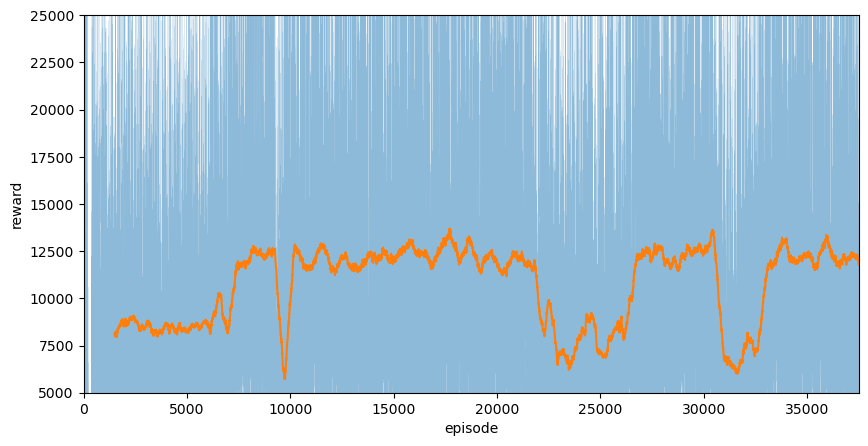
\includegraphics[width=0.8\linewidth]{fig-rainbow.png}
	\caption{Rainbow在VideoPinball-ramNoFrameskip-v4环境下的表现}
	\label{fig:rainbow}
\end{figure}


图\ref{fig:rainbow}中横轴代表进行的游戏局数,纵轴代表游戏的得分,图中背景的蓝色曲线代表每一局游戏的得分原始数据曲线,由于每一局游戏的得分波动极大,为方便看出整体趋势,我对原始数据进行了滑动平均处理,结果为图中的橙色曲线。可以看出,虽然在训练过程中仍然存在较大的波动,我们的模型整体上呈现出上升趋势,模型在与环境的交互过程中逐渐学到了更好的策略。

然后,我还设计了消融实验,测试Rainbow中的每一种改进方法对模型性能的影响。我将Rainbow中的每一种改进方法分别去除,然后在VideoPinball-ramNoFrameskip-v4环境下进行测试,每个模型训练10000局游戏,由于训练轮数较少,我增大了训练前期随机探索的概率,这导致曲线可能出现更大的波动。消融实验的结果如图\ref{fig:rainbow-ablation}所示。

\begin{figure}[htbp]
	\centering
	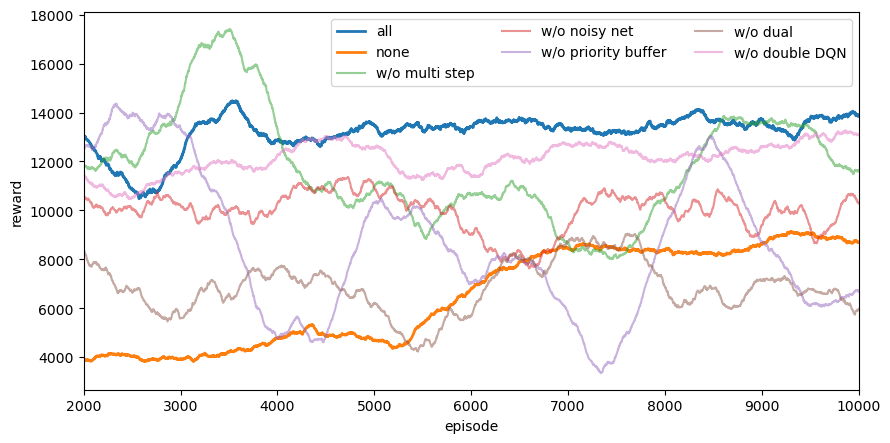
\includegraphics[width=0.9\linewidth]{fig-rainbow-ablation.png}
	\caption{Rainbow中改进方法对模型性能的影响}
	\label{fig:rainbow-ablation}
\end{figure}

图\ref{fig:rainbow-ablation}中,all曲线表示使用了我实现的所有改进方法的模型表现,none曲线为原始DQN方法模型的表现,其余曲线代表去除单个改进方法后模型的表现。可以看到,在5000局游戏之后,采用了全部改进方法的模型获得了最好的表现。原始DQN在一开始时表现最差,但是随着训练轮数增加,其表现有一个较为稳定的提升,最终超过了部分其他模型。

图\ref{fig:rainbow-ablation}中曲线波动较大,为了更直观展示出模型之间的性能差异,我根据最后500/1000局游戏的平均得分绘制了条形统计图,如图\ref{fig:rainbow-ablation-bar}所示,图中可以较为直观的看出不同模型之间的差异。

\begin{figure}[htbp]
	\centering
	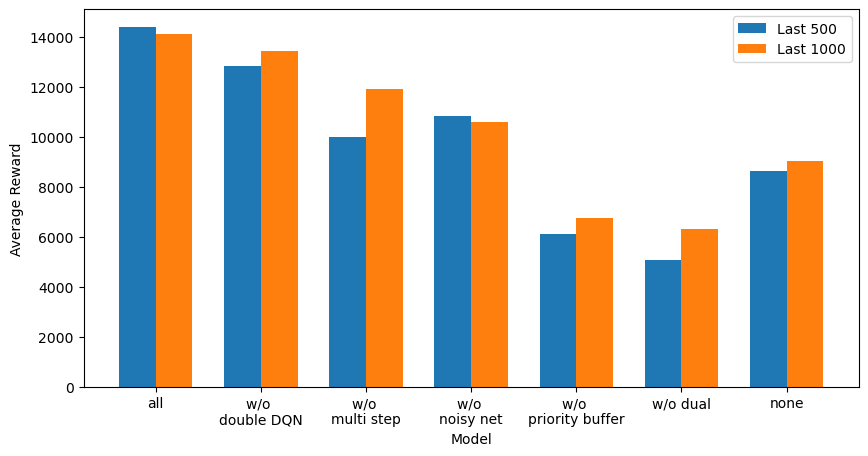
\includegraphics[width=0.9\linewidth]{fig-rainbow-ablation-bar.png}
	\caption{Rainbow中改进方法对模型性能的影响}
	\label{fig:rainbow-ablation-bar}
\end{figure}

我还在其他环境中测试了我实现的算法,图\ref{fig:rainbow-breakout-cv}是在BreakoutNoFrameskip-v4环境下的测试结果,由于图像版本的环境需要消耗大量计算量在模型的卷积部分,计算量过大导致训练缓慢,而这部分本身和强化学习没有太大关系,难以测试出模型随着与环境交互次数增加的性能变化。

\begin{figure}[htbp]
	\centering
	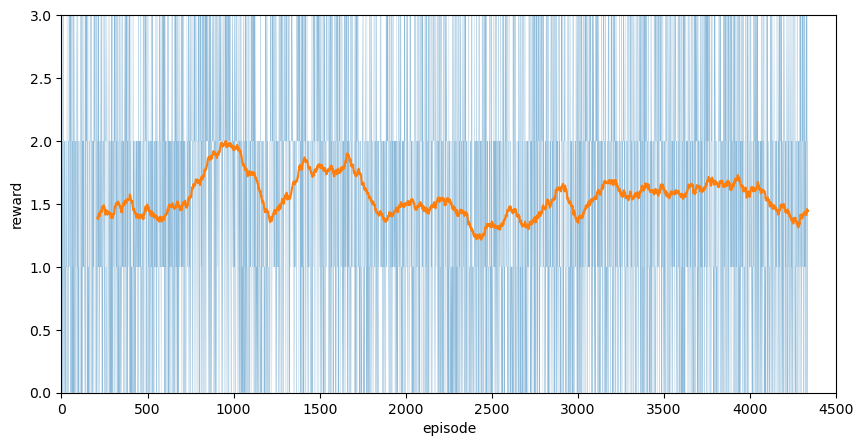
\includegraphics[width=0.9\linewidth]{fig-rainbow-breakout-cv.png}
	\caption{BreakoutNoFrameskip-v4环境测试结果}
	\label{fig:rainbow-breakout-cv}
\end{figure}

出于计算量考虑,我改用了ram版本的环境,图\ref{fig:rainbow-breakout}和图\ref{fig:rainbow-pong}分别展示了Breakout-ramNoFrameskip-v4和Pong-ramNoFrameskip-v4环境下的测试结果。模型与每个环境交互50000局游戏。

\begin{figure}[htbp]
	\centering
	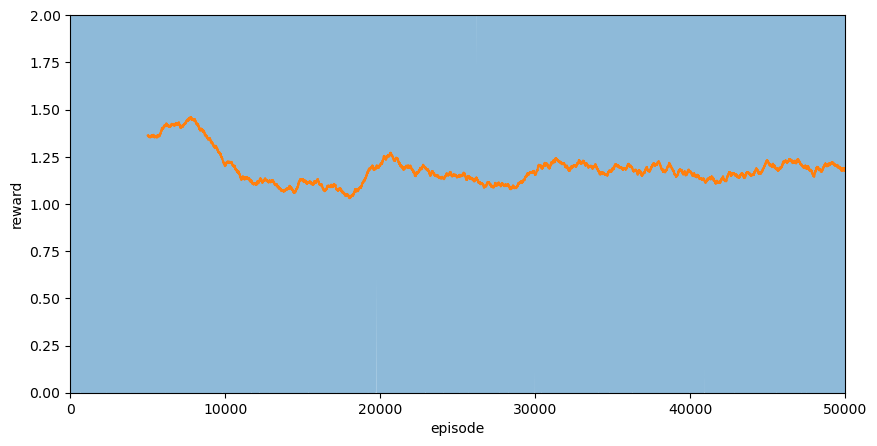
\includegraphics[width=0.9\linewidth]{fig-rainbow-breakout.png}
	\caption{Breakout-ramNoFrameskip-v4环境测试结果}
	\label{fig:rainbow-breakout}
\end{figure}

\begin{figure}[htbp]
	\centering
	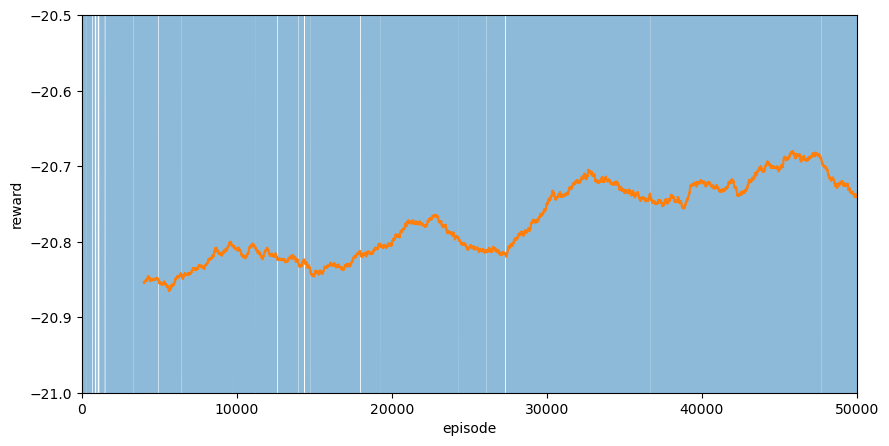
\includegraphics[width=0.9\linewidth]{fig-rainbow-pong.png}
	\caption{Pong-ramNoFrameskip-v4环境测试结果}
	\label{fig:rainbow-pong}
\end{figure}

从图\ref{fig:rainbow-breakout}看到,我们的模型在Breakout-ramNoFrameskip-v4环境下的表现并不理想,训练开始便出现了一次性能下降,后续表现虽然有缓慢的提升的迹象,但整体提升不明显。相比之下,模型在Pong-ramNoFrameskip-v4环境下的表现要好不少,从图\ref{fig:rainbow-pong}中可以明显看到模型的性能有一个较为稳定的提升趋势;但是我们也必须指出,注意到纵坐标的得分,虽然有稳定的提升趋势,这个模型的表现依然是非常差的。

我的强化学习模型在Breakout与Pong游戏中的表现明显差于VideoPinball游戏,我认为可能得原因包括:

\begin{itemize}
	\item VideoPinball状态相较于其余游戏更为简单,模型只需要关注弹球的位置,而Breakout与Pong游戏不仅有大量状态变化,还可能存在对手。
	\item VideoPinball游戏拥有更高容错率,少量错误决策对游戏的影响较小甚至完全没有影响,而Breakout与Pong游戏对错误决策非常敏感。
	\item VideoPinball游戏决策之间的时序关联性较弱,模型只需要关注当前帧做出决策,不需提前为后续状态行动。Breakout与Pong游戏都需要移动“球拍”,这需要模型提前做出正确决策。
	\item VideoPinball游戏中的模型有更多机会进行探索,因为对于VideoPinball游戏而言,完全随机动作也可以获得较高的得分,模型有更多机会接触到新的状态和动作。而Breakout与Pong游戏中,完全随机动作几乎不可能获得高分,模型的探索性较差。
\end{itemize}

模型提升缓慢是上述所有环境的共同特点,这也是强化学习面临的一大挑战。由于本项目要求必须使用model-free方法,我们的模型只能等待环境给出的奖励,但奖励可能是稀疏且滞后的,这导致模型非常难评估单个动作的好坏,因此模型的学习速度非常慢。如果允许使用model-based方法,我们可以根据对环境的理解,人为加入奖励,定向诱导模型向正确的方向学习,这样可以大大提高模型的学习速度。

\section{Policy-based Reinforcement Learning}

\subsection{方法}
基于策略的强化学习是一种强化学习方法,其核心思想是通过对策略进行建模和估计,以此为依据制定策略。在训练阶段,其学习目标是学到一个函数,知道当前状态之后,这个函数可以输出状态下每个动作的概率,记为策略。在决策阶段,我们可以根据训练好的函数,在一个新的状态下,根据策略来选择动作。

相较于基于价值的强化学习,基于策略的强化学习不需要估计Q值函数便可以直接估计出策略,因此可以用于连续决策空间问题的策略预测。

\subsubsection{Policy Gradient}

对于给定的决策模型参数$\theta$,在任意状态下,决策模型会给出选择每个动作的概率,记为$\pi_{\theta}(a|s)$,同时采取每个动作之后可以获得$R(s,a)$的收益。对于一个状态$s$,当前决策模型的期望收益可以表示为:

\begin{equation}
R_{\theta}(s) = \sum_{a} R(s,a)p_{\theta}(a|s)
\end{equation}

我们的优化目标位最大化期望收益,上式中动作的收益$R(s,a)$与决策模型无关,因此我们需要优化$p_{\theta}(a|s)$。对$R_{\theta}$求梯度有


\begin{align}
	\nabla R_{\theta} =& \sum_{a} R(s,a)\nabla p_{\theta}(a|s) \\
	=& \sum_{a} R(s,a)p_{\theta}(a|s) \frac{\nabla p_{\theta}(a|s)}{p_{\theta}(a|s)}\\
	=& \sum_{a} R(s,a)p_{\theta}(a|s)\nabla\log p_{\theta}(a|s)
	\label{eq:policy-gradient}
\end{align}
使用梯度下降更新参数,其中$\eta$为学习率:
\begin{equation}
\theta \leftarrow \theta + \eta \nabla R_\theta
\end{equation}

\subsubsection{Actor-Critic}

在等式\ref{eq:policy-gradient}中,我们需要正确计算出动作的收益$R(s,a)$才能正确更新模型。然而,我们不仅需要关注单步动作的奖励,还需考虑后续状态的价值,如果使用蒙特卡洛方法进行估计,则有$R(s,a)=\sum_{t'=t}^{T} \gamma^{t'-t} r_{t'}$。在实际问题中,这要求我们必须等到整个序列结束后才能进行更新,也要求任务必须在有限步内结束。

Actor-Critic方法借鉴基于价值的强化学习,尝试使用模型对$R(s,a)$的值进行估计。Actor-Critic方法将决策模型分为两部分:Actor用于估计策略,Critic用于估计价值。

在Actor-Critic方法方法下,$R(a,s)$可以写为:
\begin{equation}
R(a,s) = r + \gamma V(s') - V(s)
\end{equation}
其中$r$为状态$s$下行动$a$带来的即时奖励,$V$为Critic模型,$V(s)$为状态$s$的价值,$V(s')$为状态$s'$的价值。

记Critic模型的参数为$\omega$,其损失函数为
\begin{equation}
	L(\omega) = \frac{1}{2} (r + \gamma V_\omega(s_{t+1}) - V_\omega(s_t))^2
\end{equation}
其梯度为:
\begin{equation}
	\nabla_\omega L(\omega) = -(r + \gamma V_\omega(s_{t+1}) - V_\omega(s_t))\nabla_\omega V_\omega(s_t)
\end{equation}

\subsubsection{Deep Deterministic Policy Gradient}

DDPG是一种基于策略的强化学习方法。与Policy Gradient、Actor-Critic不同,DDPG是一种确定性的策略,即在给定状态下,DDPG会输出一个确定的动作,而不是一个动作的概率分布,这使得DDPG可以用于连续动作空间的问题。此外,DDPG还是一种off-policy的方法,即与环境交互的策略和更新的策略可以不同,这提高了DDPG的训练效率。

DDPG和Actor-Critic一样使用了两个模型分别估计策略和价值。为了避免价值估计模型高估价值的问题,DDPG使用了与Double Q-learning类似的方法,即使用两套模型轮流进行更新。

\subsection{实验}

我在多个环境下测试了我实现的DDPG算法。HalfCheetah-v4环境下的测试结果见图\ref{fig:ddpg-halfcheetah}。Ant-v4环境下的测试结果见图\ref{fig:ddpg-ant}。Hopper-v4环境下的测试结果见图\ref{fig:ddpg-hopper}。Humanoid-v4环境下的测试结果见图\ref{fig:ddpg-humanoid}。

\begin{figure}
	\centering
	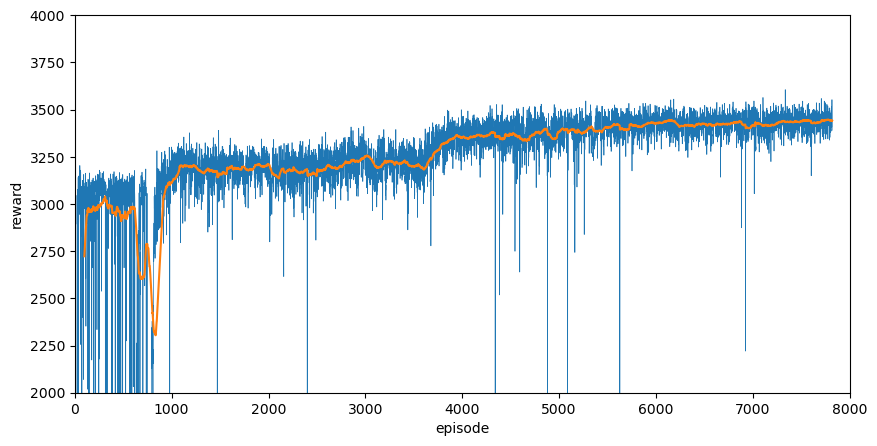
\includegraphics[width=0.9\linewidth]{fig-halfcheetah.png}
	\caption{HalfCheetah-v4环境测试结果}
	\label{fig:ddpg-halfcheetah}
\end{figure}

\begin{figure}
	\centering
	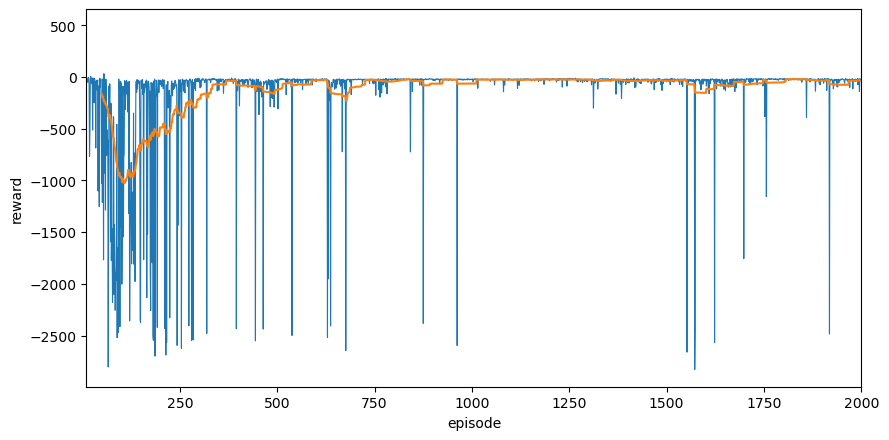
\includegraphics[width=0.9\linewidth]{fig-ant.png}
	\caption{Ant-v4环境测试结果}
	\label{fig:ddpg-ant}
\end{figure}

\begin{figure}
	\centering
	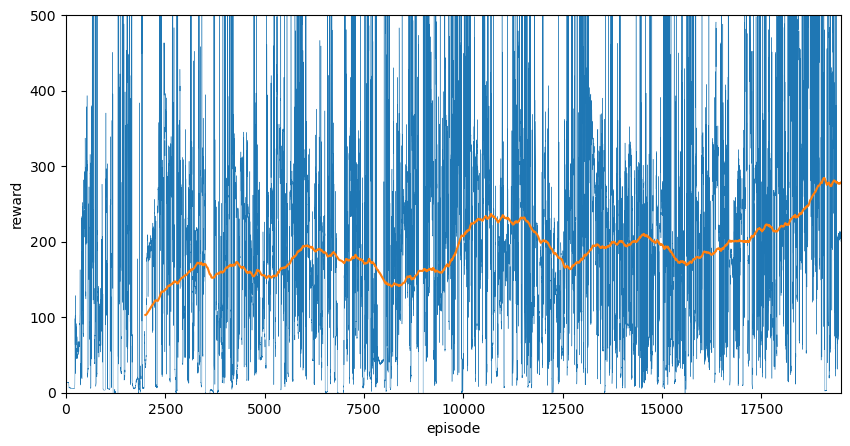
\includegraphics[width=0.9\linewidth]{fig-hopper.png}
	\caption{Hopper-v4环境测试结果}
	\label{fig:ddpg-hopper}
\end{figure}

\begin{figure}
	\centering
	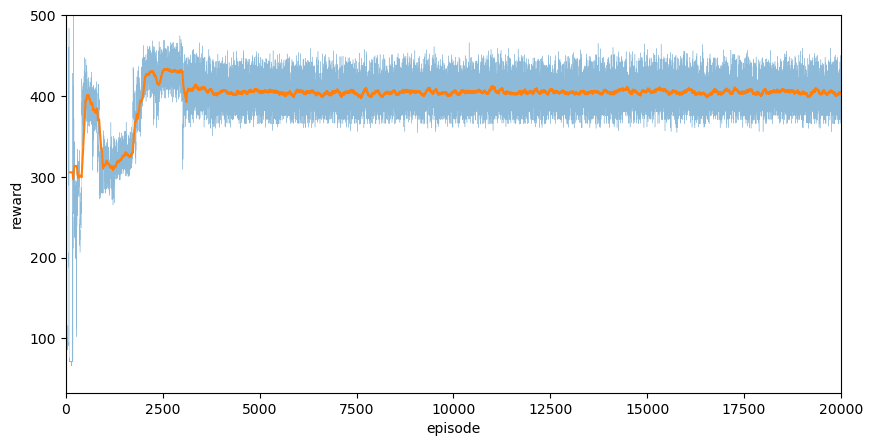
\includegraphics[width=0.9\linewidth]{fig-humanoid.png}
	\caption{Humanoid-v4环境测试结果}
	\label{fig:ddpg-humanoid}
\end{figure}

整体上看,DDPG在所有测试环境下都取得了不错的表现,随着与环境交互轮数增加,模型表现呈现出提升趋势。而不同环境之间也存在一些差异,例如图\ref{fig:ddpg-hopper}中,每一局游戏的得分波动较大,只能从平滑曲线中看出整体平均得分在上升。图\ref{fig:ddpg-ant}与图\ref{fig:ddpg-humanoid}中,在游戏轮数达到一定值后,模型提升趋势出现停滞现象,这可能是因为随着轮数增加,模型随机性降低,模型探索范围减小,导致模型陷入局部最优解,一种可能的改进方案是当检测到模型提升停滞时,强制增大模型决策的随机性,让模型有更多机会探索新的状态和动作。

\end{document}
